\section{Formaciones}
En este apartado se comentará como se ha abordado la implementación de las distintas formaciones de NPCs. Estas formaciones serán formaciones basadas en dos estructuras fijas preestablecidas con un número de huecos o slots fijo.\\

Para programar esta funcionalidad se han creado 4 clases distintas. Por un lado tenemos la clase \textit{Formation} que será la clase padre que defina los métodos que deben tener el resto de clases que hereden de esta, al igual que define las distintas formaciones que soporta.
\lstinputlisting[linerange=5-9, firstnumber=5]{\ScriptsPath/Steering/Formaciones/Formation.cs}


En esta clase además se definen dos variables clave:
\begin{itemize}
    \item \_numSlots: Representa el número de huecos de la formación.
    \item \_formationPattern: Será el patrón de formación a implementar, y tendrá uno de los valores visto en el código anterior.
\end{itemize}

Veamos dentro de esta clase cuáles son las funciones más destacadas:
\begin{itemize}
    \item GetSlotLocation(): Este método será utilizado para que un NPC a partir del número de slot que se le ha asignado, conozca cuál es la posición de su slot. Este método lo sobreescribirán las clases \textit{hijas} acorde a la formación a realizar.
    \item SupportsSlots: Este método nos permitirá conocer si queda algún slot libre dentro de la formación.
\end{itemize}

Las clases que heredan de esta clase \textit{Formation} son: \textit{FormationTriangulo} y \textit{FormationColumnas}.\\
La clase FormationTriangulo define una formación fija de 7 slots en forma de cuña como se puede ver en la Figura \ref{fig:cuña}
\begin{figure}[H]
    \centering
    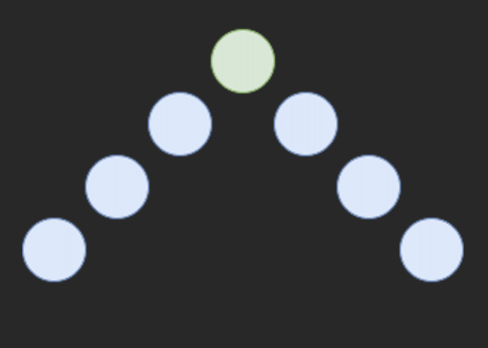
\includegraphics[scale=0.7]{formaciones/Screenshot 2022-04-01 at 19.03.11.png}
    \caption{Formación cuña}
    \label{fig:cuña}
\end{figure}
Al crear un objeto de esta clase se inicilizan las variables numSlot a 7 y el formationPattern a Triangulo quedando así definida la estructura fija de la formación. Esta clase además se encarga de redefinir la función que devuelve el Slot correspondiente a cada NPC de la siguiente forma:
\lstinputlisting[linerange=17-36, firstnumber=17]{\ScriptsPath/Steering/Formaciones/FormationTriangulo.cs}

Como podemos ver se iniciliza un Steering y este será devuelvo si el Slot es 0 lo que significa que es la posición del líder. En caso contrario se calcula la posición vertical y horizontal y se obtiene el vector posición para este NPC con las coordenadas X como producto de ambas posiciones, y a 0 y z con el valor vertical a negativo. Así ya tenemos calculado tanto la posición como la rotación del personaje.\\

La clase formationColumnas es parecida a la anterior solo que en este caso el numero de slots es 8 y formarán como se ve en la figura \ref{fig:cols}
\begin{figure}
    \centering
    
\includegraphics[scale=0.7]{formaciones/Screenshot 2022-04-01 at 19.03.24.png}
    \caption{Formación columnas}
    \label{fig:cols}
\end{figure}
Al crear un objeto de esta clase se inicilizará el numero de slotsy la distancia entre NPCs será mayor respecto a la de formación en cuña (Aunque este valor se puede cambiar en el editor). La función GetSlot Location como podemos ver es diferente, ya que en este caso se comprueba dependiendo del slot asignado si el NPC está en izquierda o derecha y si es el ultimo slot será el encargado de formar en el pico de la formación.

\lstinputlisting[linerange=18-49, firstnumber=18]{\ScriptsPath/Steering/Formaciones/FormationColumnas.cs}


Por último la clase más importante dentro del apartado de formaciones sería la del \textbf{FormationManager} donde destacan los siguientes atributos: 
\lstinputlisting[linerange=10-15, firstnumber=10]{\ScriptsPath/Steering/Formaciones/FormationManager.cs}

Estos atributos nos permitirán llevar un registro de los SlotAssignment que es una estructura auxiliar creada que consta de un Agente y el número de slot asignado a el. Luego tenemos un agente lider, el patrón a realizar y un booleano que indicará si la formación se ha realizado. La variable \textit{\_newPoint} se comentará mas adelante ya que se usa para arreglar un fallo encontrado.\\

Ahora haremos un repaso por los métodos implementados, entrando más en detalle en aquellos que son más complejos.\\

Para actualizar la lista de SlotAssignmetn tenemos dos métodos: \textbf{AddCharacter} y \textbf{RemoveCharacter}. El primero de ellos comprobará si la formación tiene huecos libres, en caso negativo el agente quedará fuera de la formación ya que la asignación es en orden de llegada. En caso afirmativo se creará un slotAsignament para este agente y se actualizará la estructura con el metodo auxiliar \textit{UpdateSlotAssignaments.} Cabe destacar que el lider será el primer personaje seleccionado al iniciar el juego, por eso si el slot ocupado es el 0 guardaremos a este en la variable \textit{\_leader}.\\

El método de eliminar personajes de la lista es muy sencillo ya que recibe un agente y este se busca en la lista de personajes y se elimina haciendo uso de los métodos que se tienen para actualizar la estructura.\\

Como métodos auxiliares tenemos \textit{AmILeader} que comprueba si el Agente es el lider o no, \textit{UnfollowLeader} que elimina el Steering de LeaderFollowing de los personajes que hay formados y \textit{LeaderAtNewPoint} que comprueba si el lider está o no en el punto al que se le ha ordenado ir.\\

El método más importante es el de \textit{Update Slots} que coge como punto de anclaje la posición del lider y su orientación y recorre la estructura de SlotAssignments como sigue: 
\lstinputlisting[linerange=92-117, firstnumber=92]{\ScriptsPath/Steering/Formaciones/FormationManager.cs}


Lo que podemos ver en estas líneas es que basicamente nos creamos un target auxiliar en la posición relativa calculada con \textit{GetSlotLocation}, y le asignaremos la posición y la orientación que debe tener dentro de la formación ya que cada personaje una vez formado tiene que tener rotación distinta a sus compañeros. Este target auxiliar se utiliza porque en un inicio se cogía la posición del líder y se tenía un error que era que cuando el lider se movía estos formaban a donde estaba líder en el momento anterior a comenzar el movimiento. Es por esto que se usa como referencia un target auxiliar igual que se hace en los Steerings Delegados.\\

Una vez calculado todo y tenemos el agente que va a moverse a ese slot, le eliminamos todos los steerings al agente exceto WallAvoidance y LookingWhereYouGoing y le añadimos los Steerings de Seek y Align que este ejecutará hacia el target.\\

Importante mencionar que la clase que inicia todo este proceso de formar es \textit{GameController} donde al pulsar la tecla \textit{F} formará como cuña y al pulsar \textit{C} formará como columnas.  Ambos métodos se implementan como sigue, cambiando solamente el tipo de Formación y la tecla a pulsar. 
\lstinputlisting[linerange=139-152, firstnumber=13]{\ScriptsPath/GameController.cs}

En el siguiente trozo de código tenemos también el arreglo del error comentado anteriormente, en este caso comprobamos que el lider se ha movido a un lugar nuevo y por tanto toca actualizar todos los Slots de la formación ya que esta está relativa a la posición del líder.

\lstinputlisting[linerange=168-175, firstnumber=168]{\ScriptsPath/GameController.cs}

Como requerimiento del cambio de posición de las formaciones se ha implementado un Steering nuevo llamado \textit{Leader Following} que será una combinación de los Steerings Arrive y Flee ya comentados anteriormente y del Steering Separation que basicamente se encarga de que el NPC se separe del resto de miembros del grupo que sigue al lider, ajustando esta separación mediante una variable que es la fuerza de repulsión. 